\documentclass[tikz,border=8pt]{standalone}
\usetikzlibrary{arrows.meta}

\begin{document}
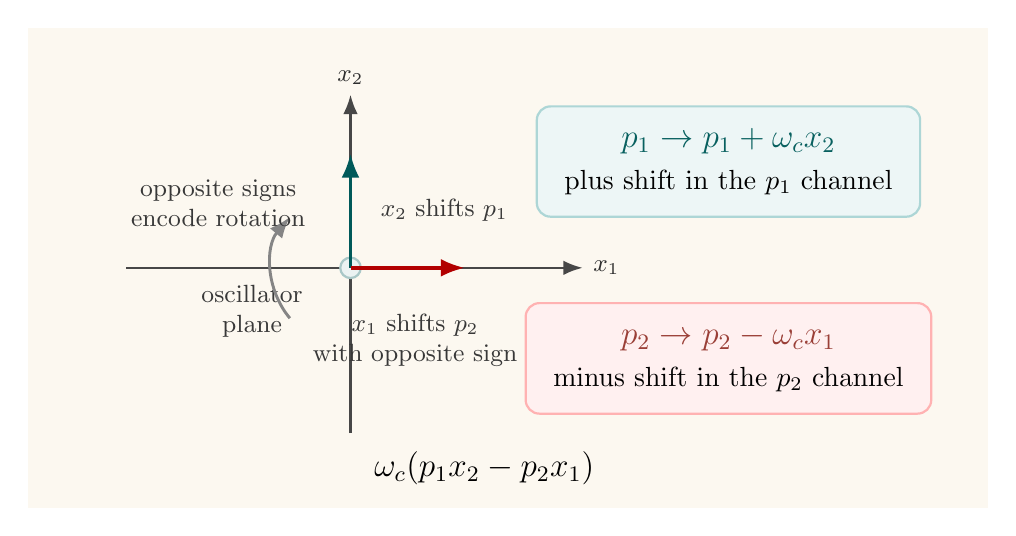
\begin{tikzpicture}[
  >=Latex,
  axis/.style={->, line width=0.9pt, draw=black!72},
  shiftarrow/.style={->, line width=1.25pt, draw=teal!70!black},
  negarrow/.style={->, line width=1.25pt, draw=red!70!black},
  note/.style={font=\small, align=center, text=black!78},
  formula/.style={font=\large, text=black},
  label/.style={font=\small\bfseries, text=black!82},
  shiftbox/.style={rounded corners=5pt, draw=teal!32, fill=teal!7, line width=0.8pt,
    inner xsep=10pt, inner ysep=8pt, align=center},
  negbox/.style={rounded corners=5pt, draw=red!30, fill=red!6, line width=0.8pt,
    inner xsep=10pt, inner ysep=8pt, align=center}
]

\definecolor{paper}{RGB}{252,248,240}
\definecolor{accent}{RGB}{8,96,95}
\definecolor{softred}{RGB}{154,63,55}

\fill[paper] (-6.1,-3.05) rectangle (6.1,3.05);

\coordinate (O) at (-2,0);

\draw[axis] (-4.85,0) -- (0.95,0) node[right,label] {$x_1$};
\draw[axis] (-2,-2.1) -- (-2,2.2) node[above,label] {$x_2$};

\draw[fill=accent!8, draw=accent!35, line width=0.8pt] (O) circle (0.13);
\node[note] at (-3.25,-0.55) {oscillator\\plane};

\draw[shiftarrow] (O) -- (-2,1.45)
  node[midway, right=7pt, note] {$x_2$ shifts $p_1$};
\draw[negarrow] (O) -- (-0.55,0);
\node[note] at (-1.18,-0.92) {$x_1$ shifts $p_2$\\with opposite sign};

\node[shiftbox] (plus) at (2.8,1.35)
  {{\large\color{accent}$p_1\rightarrow p_1+\omega_c x_2$}\\[3pt]
   plus shift in the $p_1$ channel};
\node[negbox] (minus) at (2.8,-1.15)
  {{\large\color{softred}$p_2\rightarrow p_2-\omega_c x_1$}\\[3pt]
   minus shift in the $p_2$ channel};

\draw[->, line width=1.05pt, draw=black!48] (-2.77,-0.64)
  arc[start angle=220, end angle=140, radius=1.0];
\node[note] at (-3.68,0.82) {opposite signs\\encode rotation};

\node[formula] at (-0.3,-2.55)
  {$\omega_c(p_1x_2-p_2x_1)$};

\end{tikzpicture}
\end{document}
